% !TEX program = xelatex
% Bài báo dự án: Hệ thống đặt lịch khám, quản lý hàng đợi và hồ sơ y tế
% Định dạng bài báo khoa học hai cột (IEEEtran, khổ A4).
% Biên dịch: latexmk (đã cấu hình trong .latexmkrc) hoặc xelatex main.tex hai lần.
\documentclass[conference,a4paper,10pt]{IEEEtran}

% ---------------------------------------------------------------
% Preamble — IEEEtran + XeLaTeX/LuaLaTeX (TeX Live 2022+ / MiKTeX / Overleaf)
% ---------------------------------------------------------------

% Ngôn ngữ và phông chữ
\usepackage{fontspec}
\usepackage{babel}
\babelprovide[main,import]{vietnamese}
% TeX Gyre Termes (giống Times, phông chuẩn của IEEE) hỗ trợ đầy đủ tiếng Việt.
% Gọi theo tên file để chạy được cả trên TeX Live, Overleaf và Tectonic.
\setmainfont{texgyretermes}[Extension=.otf,
  UprightFont=*-regular, BoldFont=*-bold,
  ItalicFont=*-italic, BoldItalicFont=*-bolditalic]
\setsansfont{texgyreheros}[Extension=.otf,
  UprightFont=*-regular, BoldFont=*-bold,
  ItalicFont=*-italic, BoldItalicFont=*-bolditalic]
\setmonofont{DejaVuSansMono}[Extension=.ttf, Scale=0.85,
  BoldFont=*-Bold, ItalicFont=*-Oblique, BoldItalicFont=*-BoldOblique]

% Bảng
\usepackage{booktabs}
\usepackage{tabularx}
\usepackage{multirow}
\usepackage{array}
\usepackage[table]{xcolor}
\newcolumntype{L}[1]{>{\raggedright\arraybackslash}p{#1}}
\newcolumntype{R}{>{\raggedleft\arraybackslash}X}
\newcolumntype{Y}{>{\raggedright\arraybackslash}X}
\renewcommand{\arraystretch}{1.2}

% Hình, sơ đồ, biểu đồ
\usepackage{graphicx}
\usepackage{tikz}
\usetikzlibrary{positioning,arrows.meta,fit,shapes.geometric,shapes.multipart,calc,backgrounds}
\usepackage{pgfplots}
\pgfplotsset{compat=1.18}

% Mã nguồn
\usepackage{listings}
\lstset{
  basicstyle=\ttfamily\scriptsize,
  breaklines=true,
  frame=tb,
  framerule=0.4pt,
  rulecolor=\color{black!40},
  backgroundcolor=\color{black!3},
  numbers=none,
  keywordstyle=\color{blue!60!black}\bfseries,
  commentstyle=\color{green!40!black}\itshape,
  stringstyle=\color{red!50!black},
  columns=fullflexible,
  keepspaces=true,
  showstringspaces=false,
  aboveskip=6pt,
  belowskip=4pt,
  captionpos=t,
  abovecaptionskip=0pt,
  belowcaptionskip=6pt
}
\renewcommand{\lstlistingname}{Đoạn mã}
% IEEEtran in chú thích với khoảng âm nên chú thích của listings bị đè lên khung.
% Dùng chú thích riêng: \codecaption{nội dung}{nhãn} đặt ngay trước lstlisting.
\newcounter{codelisting}
\newcommand{\codecaption}[2]{%
  \par\smallskip\refstepcounter{codelisting}\label{#2}%
  {\centering\footnotesize \lstlistingname~\thecodelisting. #1\par}\nobreak\vspace{2pt}\nobreak}

% Danh sách, liên kết, đường dẫn
\usepackage{enumitem}
\setlist{itemsep=1pt,topsep=3pt,leftmargin=*}
\usepackage{url}
\usepackage[hidelinks]{hyperref}

% Giảm giãn chữ ở cột hẹp khi dòng chứa tên mã/đường dẫn dài
\setlength{\emergencystretch}{2em}
\pgfplotsset{/pgf/number format/1000 sep={.}, /pgf/number format/use comma}

% Danh sách căn trái cho các mục chứa nhiều tên mã
\newenvironment{codeitems}{\begin{itemize}\raggedright}{\end{itemize}}

% Lệnh tiện ích
\newcommand{\code}[1]{\texttt{#1}}
\newcommand{\commitmain}{\code{5dd739f}}
\newcommand{\commitmono}{\code{1e64bfc}}

% Màu dùng chung cho sơ đồ
\definecolor{svc}{HTML}{DCEBFA}
\definecolor{svcborder}{HTML}{2F6DB5}
\definecolor{infra}{HTML}{FCEBD5}
\definecolor{infraborder}{HTML}{C07A1B}
\definecolor{obs}{HTML}{E6F2E1}
\definecolor{obsborder}{HTML}{4C8A3A}
\definecolor{mono}{HTML}{8A8F98}
\definecolor{micro}{HTML}{2F6DB5}

\tikzset{
  box/.style={draw=svcborder,fill=svc,rounded corners=2pt,align=center,
              minimum height=9mm,inner sep=4pt,font=\small},
  infrabox/.style={box,draw=infraborder,fill=infra},
  obsbox/.style={box,draw=obsborder,fill=obs},
  db/.style={cylinder,shape border rotate=90,aspect=0.18,draw=infraborder,
             fill=infra,align=center,minimum height=12mm,inner sep=3pt,font=\small},
  actor/.style={draw=black!60,fill=black!5,rounded corners=6pt,align=center,
                minimum height=8mm,inner sep=4pt,font=\small},
  arr/.style={-{Stealth[length=2.2mm]},thick,draw=black!70},
  dasharr/.style={arr,dashed},
  lbl/.style={font=\scriptsize,fill=white,inner sep=1.5pt}
}


\begin{document}

\title{Chuyển đổi hệ thống đặt lịch khám, hàng đợi\\và hồ sơ y tế từ monolith sang microservices:\\thiết kế, hiện thực và đánh giá hiệu năng}

% Thành viên 1: điền họ tên, MSSV và email vào các chỗ trống.
\author{
  \IEEEauthorblockN{\rule{4cm}{0.4pt}}
  \IEEEauthorblockA{MSSV: \rule{2.5cm}{0.4pt}\\
                    Email: \rule{4cm}{0.4pt}}
  \and
  \IEEEauthorblockN{Lê Tuấn Cảnh}
  \IEEEauthorblockA{MSSV: 23020013\\
                    Email: \href{mailto:23020013@vnu.edu.vn}{23020013@vnu.edu.vn}}
}

\maketitle
\thispagestyle{plain}
\pagestyle{plain}

\begin{abstract}
Bài báo trình bày quá trình chuyển đổi một hệ thống quản lý phòng khám (đặt lịch khám, hàng đợi tiếp đón, hồ sơ y tế và thông báo) từ kiến trúc monolith sang microservices. Hệ thống mới gồm một API Gateway và sáu service phân chia theo bounded context, mỗi service sở hữu database logic riêng và giao tiếp qua HTTP hoặc RabbitMQ. Tính nhất quán dữ liệu xuyên service được bảo đảm bằng transactional outbox, inbox, idempotency key và SAGA có hành động bù; các invariant quan trọng (không overbooking, không cấp trùng số thứ tự) được ràng buộc ở tầng database. Chúng tôi định nghĩa ma trận SLI/SLO/QoS, trang bị metrics, tracing phân tán và cảnh báo, sau đó benchmark đối chứng hai kiến trúc trên cùng ngân sách 12,5 CPU. Trong kịch bản đặt lịch tải cao (30 VU, 2.400 slot), thông lượng xác nhận của hai hệ thống tương đương (khoảng 29,7--29,8 booking/giây, 0\% lỗi 5xx), nhưng p95 từ lúc gửi yêu cầu đến khi lịch hẹn được xác nhận của microservices là 762~ms so với 235~ms của monolith. Ngược lại, dưới tải hỗn hợp có hàng đợi, microservices hoàn tất 836/836 vòng đời hàng đợi trong khi monolith gặp lỗi chức năng ở luồng walk-in. Bài báo cũng báo cáo kết quả review mã nguồn, chỉ ra các rủi ro mất event ở hai consumer thiếu dead-letter queue, và thảo luận các giới hạn của phép so sánh.
\end{abstract}

\begin{IEEEkeywords}
microservices, monolith, SAGA, transactional outbox, OpenAPI, SLO, kiểm thử tải, hệ thống phòng khám
\end{IEEEkeywords}

\section{Giới thiệu}
\label{ch:intro}

\subsection{Bối cảnh và bài toán}

Một phòng khám đa khoa cần phục vụ nhiều nhóm người dùng cùng lúc: bệnh nhân tìm bác sĩ và đặt lịch; nhân viên quản lý hồ sơ bệnh nhân và ca làm; lễ tân tiếp nhận, check-in và điều phối hàng đợi; bác sĩ khám và cập nhật hồ sơ y tế; quản trị viên theo dõi vận hành. Các nghiệp vụ này có tần suất và yêu cầu khác nhau: tìm lịch trống chủ yếu là đọc, đặt lịch là ghi có tranh chấp slot, còn hàng đợi cần cập nhật gần thời gian thực.

Phiên bản đầu tiên của hệ thống là một ứng dụng monolith. Dự án này phân rã nó thành các microservices theo bounded context, đồng thời đo đạc để đánh giá cái được và cái mất của việc chuyển đổi.

\subsection{Mục tiêu}

\begin{enumerate}
  \item Phân tích hệ thống monolith hiện có, thiết kế lại thành các service sở hữu nghiệp vụ và dữ liệu riêng.
  \item Thiết kế hợp đồng API bằng OpenAPI và có cơ chế phát hiện sai lệch (drift) giữa hợp đồng và mã nguồn.
  \item Hiện thực các luồng phối hợp giữa service bằng orchestration, choreography và SAGA, bảo đảm không overbooking và không cấp trùng số thứ tự.
  \item Định nghĩa SLI/SLO/QoS, trang bị metrics, tracing, dashboard và cảnh báo.
  \item Kiểm thử tải và so sánh đối chứng với monolith trên cùng ngân sách tài nguyên.
\end{enumerate}

\subsection{Phạm vi và chức năng chính}

Hệ thống bao gồm: xác thực và phân quyền; quản lý nhân sự, chuyên khoa, ca làm; tìm slot và đặt/hủy/đổi lịch có idempotency; tiếp nhận khách walk-in; check-in và cấp số hàng đợi; gọi, bỏ qua, bắt đầu, kết thúc lượt khám theo vai trò; hồ sơ bệnh nhân và medical record gắn với \code{AppointmentId}; hộp thư thông báo và thông báo thời gian thực qua SignalR; API Gateway; health/readiness, metrics, tracing và bộ kịch bản kiểm thử tải.

Toàn bộ hệ thống được triển khai bằng Docker Compose trên một máy. Các mục tiêu chất lượng trong bài báo là mục tiêu của đồ án trên môi trường này, không phải cam kết vận hành production.

\subsection{Nguồn số liệu}

Bài báo đối chiếu mã nguồn tại commit \commitmain{} của nhánh \code{main} (microservices) và commit \commitmono{} của nhánh \code{monolith}, cùng các tài liệu thiết kế, nghiệm thu và artifact benchmark lưu trong repo. Mọi số liệu tải đều ghi ngày chạy theo artifact gốc (11/11, 17/11 và 22/11/2026).

\subsection{Cấu trúc bài báo}

Phần còn lại của bài báo được tổ chức như sau. Mục~\ref{ch:theory} trình bày cơ sở lý thuyết. Mục~\ref{ch:monolith} mô tả hệ thống monolith. Mục~\ref{ch:micro} trình bày kiến trúc microservices và các luồng phối hợp. Mục~\ref{ch:sla} định nghĩa SLA/SLO/QoS. Mục~\ref{ch:testing} trình bày kết quả kiểm thử và so sánh hiệu năng. Mục~\ref{ch:review} là kết quả review hệ thống. Mục~\ref{ch:conclusion} kết luận và nêu hướng phát triển.

\section{Cơ sở lý thuyết}
\label{ch:theory}

\subsection{Monolith và microservices}

\textbf{Monolith} triển khai các nghiệp vụ trong một ứng dụng, thường dùng chung mô hình miền và cơ sở dữ liệu. Cách này dễ chạy, dễ kiểm thử giao dịch xuyên nghiệp vụ và có ít hop mạng, nhưng các miền khó phát hành, mở rộng và chịu lỗi độc lập.

\textbf{Microservices} chia hệ thống theo bounded context: mỗi service sở hữu nghiệp vụ, dữ liệu và API của nó~\cite{newman2021,richardson2018}. Các service có thể phát hành và mở rộng riêng; đổi lại, hệ thống phải xử lý giao tiếp mạng, lỗi một phần, eventual consistency, quản lý phiên bản hợp đồng và vận hành nhiều tiến trình.

``Database per service'' có nghĩa là quyền sở hữu dữ liệu logic riêng: một service không đọc/ghi trực tiếp bảng của service khác. Trong dự án này các database vẫn nằm trên cùng một SQL Server container, không phải các máy chủ database vật lý độc lập.

\begin{table}[!t]
\centering
\caption{So sánh monolith và microservices}
\label{tab:mono-vs-micro}
\small
\begin{tabularx}{\linewidth}{@{}L{1.6cm}YY@{}}
\toprule
\textbf{Tiêu chí} & \textbf{Monolith} & \textbf{Microservices} \\
\midrule
Triển khai & Một đơn vị, đơn giản & Nhiều đơn vị, cần orchestration hạ tầng \\
Giao dịch & ACID cục bộ, dễ & Xuyên service phải dùng SAGA/outbox \\
Độ trễ & Gọi trong tiến trình & Thêm hop mạng, serialize/deserialize \\
Mở rộng & Cả ứng dụng & Từng service theo nhu cầu \\
Cô lập lỗi & Lỗi một module ảnh hưởng toàn bộ & Lỗi được giới hạn nếu thiết kế đúng \\
Vận hành & Ít thành phần & Cần observability, tracing phân tán \\
\bottomrule
\end{tabularx}
\end{table}

\subsection{Hợp đồng API và OpenAPI}

OpenAPI~\cite{openapi} mô tả endpoint, phương thức, schema request/response, lỗi và cơ chế bảo vệ API theo định dạng máy đọc được. Hợp đồng giúp frontend, Gateway và service thống nhất cách tích hợp, sinh tài liệu Swagger, phát hiện drift giữa schema công bố và implementation, và làm căn cứ cho contract testing. Hợp đồng không tự chứng minh API hoạt động đúng; vẫn cần kiểm thử tích hợp và runtime.

\subsection{Orchestration, choreography và SAGA}

\begin{itemize}
  \item \textbf{Orchestration:} một thành phần điều phối các bước nghiệp vụ và biết bước tiếp theo cần gọi. Dễ thấy luồng tổng thể, nhưng điều phối viên có thể trở thành nơi tập trung logic.
  \item \textbf{Choreography:} các service phản ứng với event do service khác phát ra; không có bộ điều phối trung tâm. Các service ít phụ thuộc trực tiếp hơn, nhưng cần observability và quản lý event tốt.
  \item \textbf{SAGA}~\cite{garcia1987sagas}: giao dịch nghiệp vụ dài được tách thành chuỗi giao dịch cục bộ. Nếu bước sau thất bại, hệ thống retry hoặc thực hiện hành động bù thay vì giữ một transaction ACID xuyên nhiều database.
  \item \textbf{Transactional outbox / inbox và idempotency}~\cite{richardson2018}: outbox ghi thay đổi nghiệp vụ và event cần phát trong cùng transaction cục bộ; publisher gửi lại khi broker phục hồi. Inbox và idempotency key chặn event hoặc request lặp gây tác dụng phụ trùng.
\end{itemize}

\subsection{SLA, SLI, SLO và QoS}

Theo cách tiếp cận Site Reliability Engineering~\cite{beyer2016sre}:

\begin{itemize}
  \item \textbf{SLI} là chỉ số đo thực tế, ví dụ tỷ lệ request hợp lệ không lỗi 5xx hoặc độ trễ p95.
  \item \textbf{SLO} là mục tiêu nội bộ cho SLI trong một cửa sổ và mẫu đo đã định nghĩa.
  \item \textbf{SLA} là cam kết với khách hàng, thường kèm trách nhiệm khi vi phạm. Ma trận trong dự án là mục tiêu nghiệm thu của đồ án, không phải hợp đồng SLA.
  \item \textbf{QoS} là các chính sách phục vụ như timeout, rate limit, retry, giới hạn đồng thời, idempotency và xử lý quá tải.
\end{itemize}

\section{Hệ thống monolith cũ}
\label{ch:monolith}

\subsection{Kiến trúc và triển khai}

Monolith (nhánh \code{monolith}) là một ứng dụng ASP.NET Core (\code{Clinic.API}) chia lớp API / Application / Domain / Infrastructure, đi kèm frontend Vue và một SQL Server. Các nghiệp vụ gọi nhau trong cùng tiến trình và dùng một \code{ApplicationDbContext} duy nhất (Hình~\ref{fig:monolith}). Đây là khác biệt chính so với ranh giới sở hữu dữ liệu của bản microservices.

Để benchmark đối chứng, monolith được container hóa bằng \path{docker-compose.monolith.yml} (API ở cổng 5100) với tổng ngân sách CPU tương đương bản microservices (12,5 CPU).

\begin{figure}[!t]
\centering
\resizebox{\linewidth}{!}{%
\begin{tikzpicture}[node distance=9mm and 12mm]
  \node[actor] (u) {Patient / Receptionist\\Doctor / Admin};
  \node[box, right=of u] (fe) {Vue Frontend};
  \node[box, right=of fe, minimum width=4.2cm] (api) {\textbf{Clinic.API (monolith)}\\Controllers + Application\\+ Domain};
  \node[box, below=of api, minimum width=4.2cm] (inf) {Infrastructure / EF Core\\\code{ApplicationDbContext}};
  \node[db, below=of inf] (db) {SQL Server\\ClinicDB};
  \draw[arr] (u) -- (fe);
  \draw[arr] (fe) -- node[lbl,above]{HTTP} (api);
  \draw[arr] (api) -- node[lbl,right]{gọi trong tiến trình} (inf);
  \draw[arr] (inf) -- (db);
\end{tikzpicture}%
}
\caption{Kiến trúc hệ thống monolith}
\label{fig:monolith}
\end{figure}

\subsection{Thiết kế cơ sở dữ liệu}

\code{ApplicationDbContext} đăng ký chung các nhóm bảng:
\begin{codeitems}
  \item \textbf{Định danh và phân quyền:} \code{Persons}, \code{Users}, \code{Roles}, \code{Permissions}, \code{UserRoles}, \code{RolePermissions}, \code{RefreshTokens}.
  \item \textbf{Nhân sự và lịch làm việc:} \code{Employees}, \code{Doctors}, \code{Specialties}, \code{WorkHistories}, \code{WorkSchedules}, \code{ShiftRequests}.
  \item \textbf{Khám bệnh:} \code{Patients}, \code{Appointments}, \code{AppointmentSnapshots}, \code{QueueTickets}, \code{QueueCounters}.
  \item \textbf{Hồ sơ y tế:} \code{MedicalReports}, \code{MedicalReportAmendments}, \code{MedicalAccessAudits}.
  \item \textbf{Thông báo:} \code{Notifications}.
\end{codeitems}

Cấu hình EF Core nằm ở \path{backend/Clinic.Infrastructure.Sqlserver/Configurations}. Hình~\ref{fig:erd} là ERD khái quát các quan hệ nghiệp vụ chính (không liệt kê mọi cột, index hay migration).

\begin{figure*}[t]
\centering
\resizebox{\linewidth}{!}{%
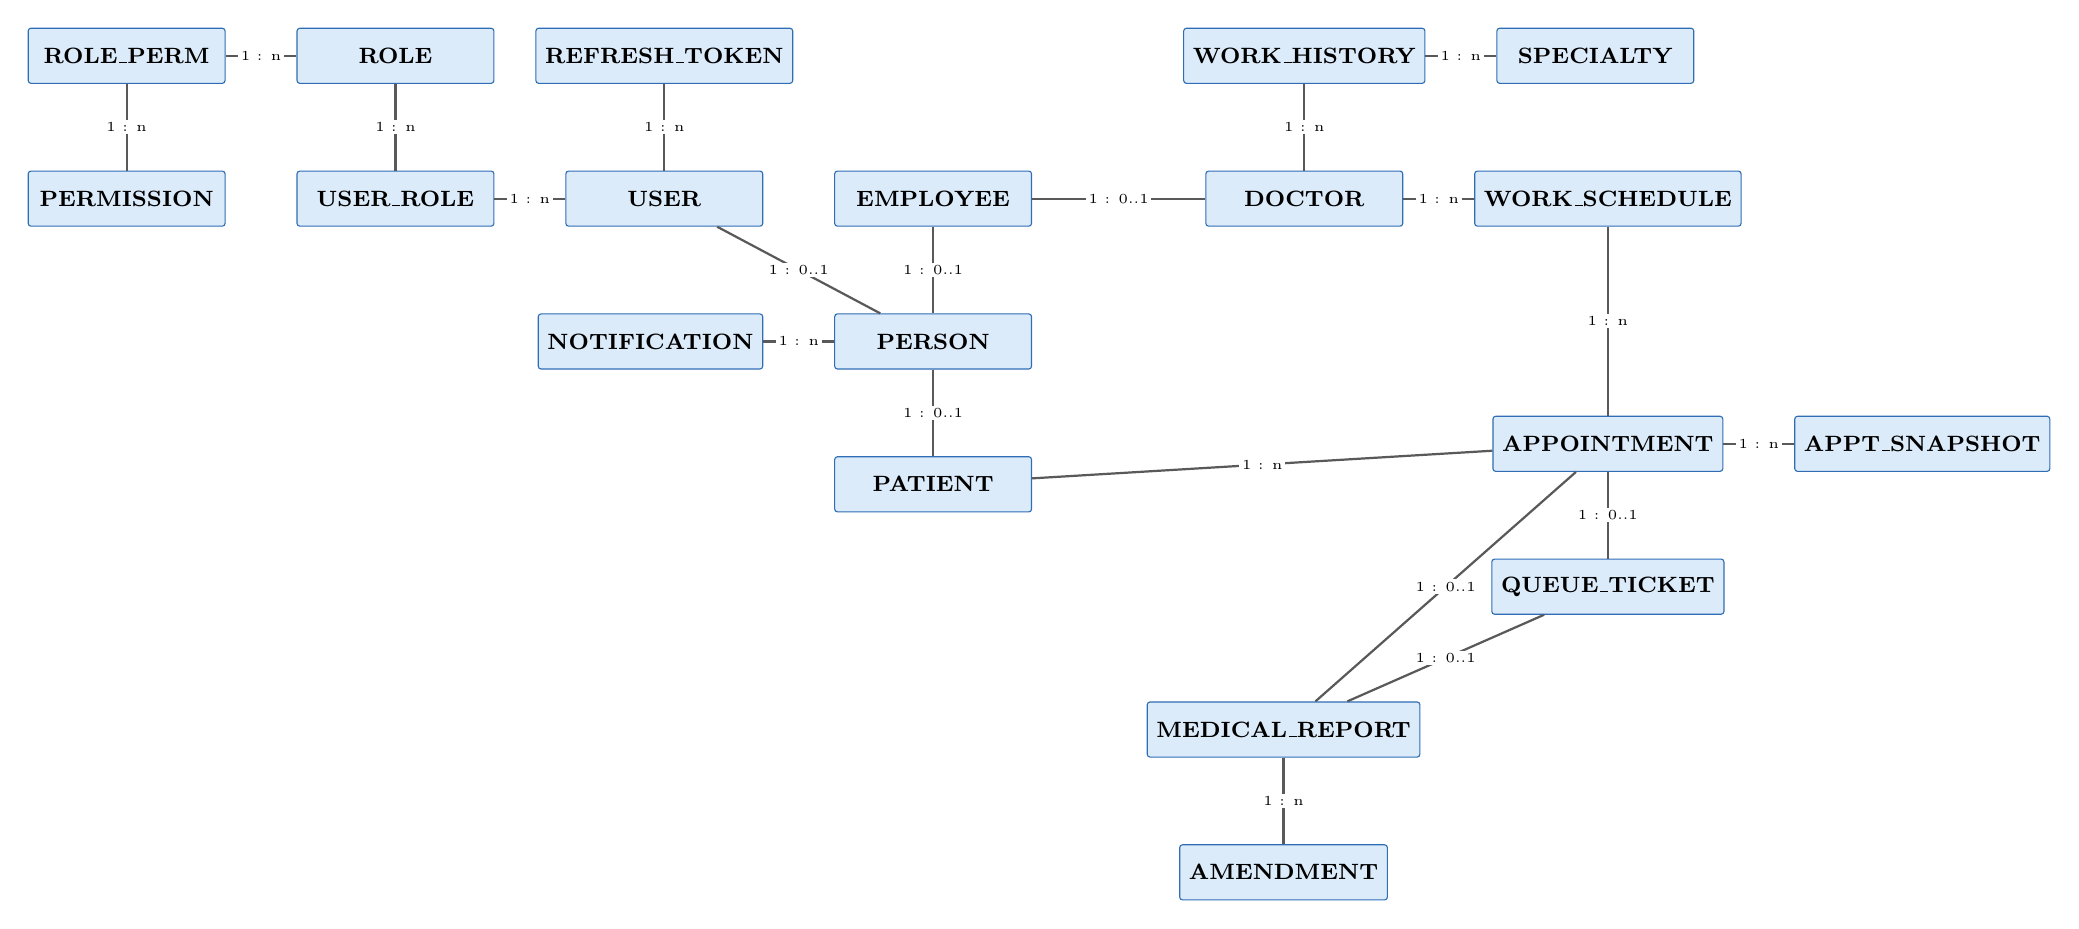
\begin{tikzpicture}[
  ent/.style={draw=svcborder,fill=svc,rounded corners=1pt,font=\footnotesize\bfseries,
              minimum width=2.5cm,minimum height=7mm,align=center},
  rel/.style={draw=black!65,thick},
  card/.style={font=\tiny,fill=white,inner sep=1pt},
  node distance=11mm and 9mm]
  % Cột giữa: Person
  \node[ent] (person) {PERSON};
  \node[ent, above left=of person] (user) {USER};
  \node[ent, above=of person] (employee) {EMPLOYEE};
  \node[ent, below=of person] (patient) {PATIENT};
  \node[ent, left=of person] (notif) {NOTIFICATION};
  % Định danh
  \node[ent, above=of user] (rtoken) {REFRESH\_TOKEN};
  \node[ent, left=of user] (userrole) {USER\_ROLE};
  \node[ent, above=of userrole] (role) {ROLE};
  \node[ent, left=of role] (roleperm) {ROLE\_PERM};
  \node[ent, below=of roleperm] (perm) {PERMISSION};
  % Nhân sự
  \node[ent, right=22mm of employee] (doctor) {DOCTOR};
  \node[ent, above=of doctor] (workhist) {WORK\_HISTORY};
  \node[ent, right=of workhist] (specialty) {SPECIALTY};
  \node[ent, right=of doctor] (schedule) {WORK\_SCHEDULE};
  % Khám
  \node[ent, below=24mm of schedule] (appt) {APPOINTMENT};
  \node[ent, right=of appt] (snap) {APPT\_SNAPSHOT};
  \node[ent, below=of appt] (ticket) {QUEUE\_TICKET};
  \node[ent, below left=of ticket] (report) {MEDICAL\_REPORT};
  \node[ent, below=of report] (amend) {AMENDMENT};

  \draw[rel] (person) -- node[card]{1 : 0..1} (user);
  \draw[rel] (person) -- node[card]{1 : 0..1} (employee);
  \draw[rel] (person) -- node[card]{1 : 0..1} (patient);
  \draw[rel] (person) -- node[card]{1 : n} (notif);
  \draw[rel] (user) -- node[card]{1 : n} (rtoken);
  \draw[rel] (user) -- node[card]{1 : n} (userrole);
  \draw[rel] (role) -- node[card]{1 : n} (userrole);
  \draw[rel] (role) -- node[card]{1 : n} (roleperm);
  \draw[rel] (perm) -- node[card]{1 : n} (roleperm);
  \draw[rel] (employee) -- node[card]{1 : 0..1} (doctor);
  \draw[rel] (doctor) -- node[card]{1 : n} (workhist);
  \draw[rel] (specialty) -- node[card]{1 : n} (workhist);
  \draw[rel] (doctor) -- node[card]{1 : n} (schedule);
  \draw[rel] (schedule) -- node[card]{1 : n} (appt);
  \draw[rel] (patient) -- node[card]{1 : n} (appt);
  \draw[rel] (appt) -- node[card]{1 : n} (snap);
  \draw[rel] (appt) -- node[card]{1 : 0..1} (ticket);
  \draw[rel] (appt) -- node[card]{1 : 0..1} (report);
  \draw[rel] (ticket) -- node[card]{1 : 0..1} (report);
  \draw[rel] (report) -- node[card]{1 : n} (amend);
\end{tikzpicture}%
}
\caption{ERD khái quát của CSDL monolith}
\label{fig:erd}
\end{figure*}

Một số quan hệ là tùy chọn: Person có thể chưa có User; khách walk-in vẫn có hồ sơ Person/Patient. \code{MedicalAccessAudits} nằm cùng database nhưng chỉ khai báo khóa và index, không khai báo khóa ngoại trong EF nên không xuất hiện trên sơ đồ.

\subsection{Hạn chế của monolith}

\begin{itemize}
  \item Mọi miền nghiệp vụ chia sẻ một mô hình dữ liệu; thay đổi schema ở một miền có thể ảnh hưởng miền khác.
  \item Không thể mở rộng riêng phần chịu tải cao (đặt lịch, hàng đợi) mà phải nhân bản toàn bộ ứng dụng.
  \item Lỗi ở một module (ví dụ gửi thông báo) có thể làm chậm hoặc làm hỏng cả tiến trình.
  \item Phát hành phải triển khai lại toàn bộ ứng dụng.
\end{itemize}

\section{Kiến trúc microservices}
\label{ch:micro}

\subsection{Phân rã nghiệp vụ}

Frontend truy cập hệ thống qua Clinic API Gateway (\code{Clinic.API} ở nhánh \code{main}; sau đợt cleanup, project này chỉ còn vai trò Gateway). Gateway xác thực, áp chính sách QoS và proxy request đến service sở hữu nghiệp vụ. Hệ thống được chia thành sáu bounded context (Bảng~\ref{tab:services}).

\begin{table*}[t]
\centering
\caption{Các service và dữ liệu sở hữu}
\label{tab:services}
\small
\begin{tabularx}{\linewidth}{@{}L{2.5cm}L{3.9cm}YL{3.8cm}@{}}
\toprule
\textbf{Service} & \textbf{Project} & \textbf{Nghiệp vụ / dữ liệu sở hữu} & \textbf{Database logic} \\
\midrule
Identity & \path{Clinic.Identity.Service} & Tài khoản, credential, token, role/permission & \code{ClinicIdentityDB} \\
Staff \& Scheduling & \path{Clinic.StaffScheduling.Service} & Nhân sự/bác sĩ, chuyên khoa, ca làm, reservation slot & \code{ClinicSchedulingDB} \\
Appointment & \path{Clinic.Appointment.Service} & Vòng đời lịch hẹn, đặt/đổi/hủy/check-in, walk-in, outbox & \code{ClinicAppointmentDB} \\
Queue & \path{Clinic.Queue.Service} & Queue ticket/counter, số thứ tự, trạng thái gọi/khám & \code{ClinicQueueDB} \\
Medical Records & \path{Clinic.MedicalRecords.Service} & Hồ sơ bệnh nhân, encounter, medical report, amendment, audit & \code{ClinicMedicalRecordsDB} \\
Notification & \path{Clinic.Notification.Service} & Inbox, delivery/outbox, replay, SignalR hub & \code{ClinicNotificationDB} \\
\bottomrule
\end{tabularx}
\end{table*}

Sáu database được cấu hình riêng nhưng cùng chạy trên service \code{db} (một SQL Server container) trong Docker Compose. Mỗi service chỉ có connection string tới database của chính nó; giao tiếp liên service đi qua HTTP client có cấu hình hoặc qua RabbitMQ.

\subsection{Sơ đồ tổng quan}

\begin{figure*}[t]
\centering
\resizebox{\linewidth}{!}{%
\begin{tikzpicture}[svc/.style={box,minimum width=2.6cm,minimum height=11mm}]
  % Lớp truy cập
  \node[actor] (users) at (0,3.2) {Patient / Receptionist / Doctor / Admin};
  \node[box] (fe) at (0,1.7) {Frontend (Vue)};
  \node[box, minimum width=8.5cm] (gw) at (0,0) {\textbf{Clinic.API Gateway}\\Public API + Auth (JWT) + QoS (rate limit) + Proxy};
  % Quan sát
  \node[obsbox, minimum width=3.2cm, minimum height=8mm] (prom)   at (8.5,0.5)  {Prometheus + alert};
  \node[obsbox, minimum width=3.2cm, minimum height=8mm] (jaeger) at (8.5,-0.5) {Jaeger (OTLP)};
  % Hàng service
  \node[svc] (id)  at (-8.5,-2.4) {Identity};
  \node[svc] (sch) at (-5.1,-2.4) {Staff \&\\Scheduling};
  \node[svc] (ap)  at (-1.7,-2.4) {Appointment};
  \node[svc] (q)   at (1.7,-2.4)  {Queue};
  \node[svc] (mr)  at (5.1,-2.4)  {Medical\\Records};
  \node[svc] (nt)  at (8.5,-2.4)  {Notification\\+ SignalR};
  % Event bus và CSDL
  \node[infrabox, minimum width=19.6cm, minimum height=8mm] (mq) at (0,-4.4)
       {\textbf{RabbitMQ} — topic exchange, retry queue, DLX};
  \node[infrabox, minimum width=9cm, minimum height=9mm, rounded corners=6pt] (sql) at (0,-6.3)
       {SQL Server container — 6 database logic (mỗi service một DB)};

  \draw[arr] (users) -- (fe);
  \draw[arr] (fe) -- (gw);
  \foreach \s in {id,sch,ap,q,mr,nt} { \draw[arr] (gw.south) -- (\s.north); }

  % Lời gọi HTTP đồng bộ Appointment <-> Scheduling
  \draw[{Stealth[length=2mm]}-{Stealth[length=2mm]},thick,draw=svcborder] (sch.east) -- node[lbl,above]{HTTP} (ap.west);

  % Event: Identity chỉ phát, các service còn lại vừa phát vừa nhận
  \draw[arr,draw=red!60!black] (id.south) -- (id.south |- mq.north);
  \foreach \s in {sch,ap,q,mr} {
    \draw[{Stealth[length=2mm]}-{Stealth[length=2mm]},thick,draw=red!60!black]
      ($(\s.south)+(-0.5,0)$) -- ($(\s.south)+(-0.5,0)$ |- mq.north);
  }
  \draw[arr,draw=red!60!black] ($(nt.south)+(-0.5,0)$ |- mq.north) -- ($(nt.south)+(-0.5,0)$);

  % Kết nối CSDL vẽ ở lớp nền, đi phía sau thanh RabbitMQ
  \begin{scope}[on background layer]
    \foreach \s in {id,sch,ap,q,mr,nt} {
      \draw[draw=infraborder!70,thick,dashed] ($(\s.south)+(0.5,0)$) -- (sql.north);
    }
  \end{scope}

  \draw[dasharr,draw=obsborder] (prom.west) -- node[lbl,above]{scrape} (gw.east |- prom.west);
  \draw[dasharr,draw=obsborder] (gw.east |- jaeger.west) -- node[lbl,below]{trace} (jaeger.west);
\end{tikzpicture}%
}
\caption{Tổng quan kiến trúc microservices. Mọi service đều được Prometheus scrape và gửi trace sang Jaeger; sơ đồ chỉ vẽ Gateway cho gọn.}
\label{fig:overview}
\end{figure*}

Hình~\ref{fig:overview} thể hiện quyền sở hữu và hướng giao tiếp logic. Mũi tên đỏ là luồng event qua RabbitMQ (Identity chỉ phát event, các service khác vừa phát vừa nhận); mũi tên xanh giữa Appointment và Scheduling là lời gọi HTTP đồng bộ; đường đứt màu cam là kết nối của từng service tới database riêng trên SQL Server dùng chung.

\subsection{Luồng đặt lịch: điều phối lai và SAGA}

Đặt lịch là luồng có tranh chấp: nhiều bệnh nhân có thể cùng chọn một slot. Hệ thống dùng \textbf{điều phối lai}: Appointment điều khiển trực tiếp các bước reserve/confirm qua API, còn việc lan truyền kết quả sang các bounded context khác dùng choreography qua event (Hình~\ref{fig:booking}).

\begin{figure*}[t]
\centering
\resizebox{\linewidth}{!}{%
\begin{tikzpicture}[
  ll/.style={draw=black!35,dashed},
  head/.style={box,minimum width=2.6cm},
  msg/.style={arr},
  ret/.style={arr,dashed,draw=black!55},
  note/.style={font=\scriptsize,align=left,fill=yellow!10,draw=yellow!50!black,inner sep=3pt}]
  \foreach \x/\n/\lab in {0/c/Client,3.4/gw/Gateway,6.8/ap/Appointment,10.2/sch/Scheduling,13.6/mq/RabbitMQ,17/nt/Notification} {
    \node[head] (\n) at (\x,0) {\lab};
    \draw[ll] (\x,-0.5) -- (\x,-12.2);
  }
  \draw[msg] (0,-1.1) -- node[lbl,above]{POST /appointments} node[lbl,below]{+ Idempotency-Key} (3.4,-1.1);
  \draw[msg] (3.4,-1.7) -- node[lbl,above]{proxy} (6.8,-1.7);
  \draw[msg] (6.8,-2.4) -- node[lbl,above]{reserve slot} (10.2,-2.4);
  \draw[ret] (10.2,-3.0) -- node[lbl,above]{reservation (10 phút)} node[lbl,below]{hoặc 409} (6.8,-3.0);
  \node[note,anchor=west] at (7.0,-3.9) {Ghi appointment (chờ xác nhận)\\+ outbox trong một transaction};
  \draw[ret] (6.8,-4.8) -- node[lbl,above]{201 Created} (3.4,-4.8);
  \draw[ret] (3.4,-5.3) -- (0,-5.3);
  \node[note,anchor=west] at (7.0,-6.2) {ConfirmationWorker (đánh thức bởi\\AppointmentWorkSignal)};
  \draw[msg] (6.8,-7.1) -- node[lbl,above]{confirm reservation} (10.2,-7.1);
  \draw[ret] (10.2,-7.7) -- node[lbl,above]{ok} (6.8,-7.7);
  \draw[msg] (6.8,-8.5) -- node[lbl,above]{AppointmentConfirmed (outbox publisher)} (13.6,-8.5);
  \draw[msg] (13.6,-9.2) -- node[lbl,above]{deliver} (17,-9.2);
  \node[note,anchor=east] at (16.8,-10.1) {Inbox chống trùng, tạo thông báo};
  \node[note,anchor=west] at (7.0,-11.3) {Lỗi confirm: retry tối đa 4 lần có backoff,\\sau đó release reservation};
\end{tikzpicture}%
}
\caption{Luồng đặt lịch: bước đồng bộ reserve và SAGA nền xác nhận}
\label{fig:booking}
\end{figure*}

\begin{enumerate}
  \item Gateway chuyển \code{POST /appointments} kèm idempotency key đến Appointment Service. Gửi lại cùng key trả về đúng lịch hẹn đã tạo.
  \item Appointment kiểm tra request và patient projection, gọi Scheduling để reserve slot. Đây là bước đồng bộ, trả \code{409} khi slot đã hết. Reservation có hạn 10 phút; \code{ReservationExpirationWorker} thu hồi reservation quá hạn.
  \item Appointment ghi lịch hẹn trạng thái chờ và outbox trong cùng transaction cục bộ.
  \item \code{AppointmentConfirmationWorker} gọi Scheduling để confirm, retry tối đa 4 lần với backoff; nếu vẫn thất bại thì release reservation (hành động bù). Khi thành công, lịch hẹn chuyển \code{Confirmed} và phát \code{AppointmentConfirmed}.
  \item Notification consume event qua inbox để tạo thông báo. Nếu broker gián đoạn, outbox giữ thông điệp đến khi broker phục hồi.
\end{enumerate}

Vì các database độc lập, đây không phải một transaction ACID xuyên hệ thống. Tính đúng đắn dựa vào khóa bản ghi schedule cùng filtered unique index ở Scheduling (chống overbooking), unique idempotency key ở Appointment (chống tạo trùng) và hành động bù khi confirm thất bại.

\textbf{Hủy lịch:} Appointment ghi trạng thái hủy và \code{AppointmentCancelled} vào outbox, đồng thời gọi trực tiếp Scheduling để nhả slot (best-effort). Scheduling cũng consume event để nhả slot, nên hai đường bổ trợ cho nhau.

\subsection{Luồng check-in và hàng đợi: choreography}

\begin{figure}[!t]
\centering
\resizebox{\linewidth}{!}{%
\begin{tikzpicture}[node distance=10mm and 14mm]
  \node[box] (ap) {Appointment};
  \node[infrabox, right=of ap] (mq) {RabbitMQ};
  \node[box, right=of mq] (q) {Queue};
  \node[box, below=14mm of mq, xshift=-38mm] (mr) {Medical Records};
  \node[box, below=14mm of mq, xshift=0mm] (nt) {Notification};
  \node[box, below=14mm of mq, xshift=38mm] (ap2) {Appointment};

  \draw[arr] (ap) -- node[lbl,above]{\scriptsize 1. CheckedIn} (mq);
  \draw[arr] (mq.north east) to[bend left=35] node[lbl,above]{\scriptsize 2. tạo ticket} (q.north west);
  \draw[arr] (q.south west) to[bend left=35] node[lbl,pos=0.35,below right]{\scriptsize 3. gọi số / khám} (mq.south east);
  \draw[arr] (mq) -- (mr);
  \draw[arr] (mq) -- (nt);
  \draw[arr] (mq) -- node[lbl,pos=0.75,left]{\scriptsize exam-completed} (ap2);
\end{tikzpicture}%
}
\caption{Choreography của luồng check-in, hàng đợi, hồ sơ và thông báo}
\label{fig:checkin}
\end{figure}

\begin{enumerate}
  \item Appointment kiểm tra check-in theo \code{AppointmentId}, ghi trạng thái và \code{AppointmentCheckedIn} vào outbox.
  \item Queue consume event qua inbox (unique index), tạo đúng một ticket cho mỗi lịch hẹn và cấp số theo ngày/bác sĩ. Lỗi tạm thời được đưa vào retry queue (tối đa 3 lần); quá số lần thì vào DLQ.
  \item Queue phát event gọi số, bắt đầu và kết thúc khám. Medical Records cập nhật encounter theo \code{AppointmentId}, Notification tạo thông báo, Appointment nhận \code{queue.exam-completed} để đóng lịch hẹn.
  \item Event trùng hoặc retry không tạo ticket/encounter trùng; thứ tự vòng đời được bảo vệ bằng state guard và idempotency.
\end{enumerate}

Hai invariant quan trọng được bảo vệ ngay tại tầng database của Queue:

\codecaption{Unique index trong QueueTicketConfiguration.cs}{lst:queue-index}
\begin{lstlisting}[language={[Sharp]C}]
// 1 ticket per appointment
builder.HasIndex(t => t.AppointmentId)
    .IsUnique()
    .HasDatabaseName("IX_QueueTickets_AppointmentId");

// Unique queue number per doctor per day
builder.HasIndex(t => new { t.DoctorId, t.QueueDate, t.QueueNumber })
    .IsUnique()
    .HasDatabaseName("IX_QueueTickets_DoctorId_QueueDate_QueueNumber");
\end{lstlisting}

\subsection{Hợp đồng API}

Repo lưu OpenAPI snapshot cho Gateway và sáu service trong \path{tasks/contracts/} (kèm \path{api-catalog-baseline.json}). Mỗi service công bố endpoint Swagger, và \code{ApiContractDriftTests} trong \path{backend/Clinic.IntegrationTests} so sánh schema đang chạy với snapshot để phát hiện drift. Lượt nghiệm thu ngày 10/11/2026 ghi contract validation 13/13 pass.

\subsection{Observability và triển khai}

\begin{codeitems}
  \item \textbf{Metrics:} mọi service xuất metrics cho Prometheus; \code{mssql-exporter} thu số liệu SQL Server. Dashboard SLA và alert rule nằm trong \path{observability/}.
  \item \textbf{Tracing:} các service gửi trace qua OTLP sang Jaeger, cho phép theo dõi một request đi qua Gateway và nhiều service.
  \item \textbf{Health:} mỗi service có health/readiness check; Compose chỉ khởi động service phụ thuộc khi service trước đã healthy.
  \item \textbf{Tài nguyên:} mỗi container có giới hạn CPU/RAM trong \path{docker-compose.yml}, tổng cộng 12,5 CPU, bằng ngân sách của monolith khi benchmark.
  \item \textbf{Bảo mật:} JWT ký bằng khóa bất đối xứng lưu trong volume; các service xác thực token qua Identity. Mật khẩu RabbitMQ bắt buộc cấu hình qua \code{.env}.
\end{codeitems}

\section{SLA, SLO và QoS}
\label{ch:sla}

\subsection{Ma trận mục tiêu}

Ma trận chi tiết nằm trong \path{tasks/SLI_SLO_MATRIX_MEMBER_A.md}. Bảng~\ref{tab:slo} tóm tắt các mục tiêu nghiệm thu chính.

\begin{table*}[t]
\centering
\caption{Các SLI/SLO và chính sách QoS}
\label{tab:slo}
\small
\begin{tabularx}{\linewidth}{@{}L{3.3cm}L{3.6cm}Y@{}}
\toprule
\textbf{SLI / QoS} & \textbf{Mục tiêu} & \textbf{Cách hiểu} \\
\midrule
Availability tại Gateway & $\geq 99{,}0\%$ & Loại các 4xx hợp lệ, 401/403, 409 tranh chấp, 429 throttling và client abort khỏi lỗi hệ thống; 5xx/502/503/504 tính là failure \\
Độ trễ API & p95 $\leq 500$ ms; p99 $\leq 1.500$ ms & Đo riêng từng endpoint/boundary; percentile các hop không cộng lại \\
Lỗi server & $\leq 1{,}0\%$ & Theo cửa sổ và mẫu tối thiểu quy định trong ma trận \\
Độ trễ xử lý event & p95 $\leq 5$ s & Từ lúc publish đến lúc xử lý/ack \\
DLQ & 0 message hợp lệ bị bỏ lại & Poison event phải được cách ly, chẩn đoán và replay an toàn \\
Invariant & 0 overbooking; 0 ticket trùng & Kiểm tra bằng integration/load test và truy vấn đối soát \\
Rate limiting & Fixed window, 100 request/phút/partition & Người dùng đã xác thực theo subject; ẩn danh theo IP \\
\bottomrule
\end{tabularx}
\end{table*}

\subsection{Hiện thực các chính sách QoS}

\begin{itemize}
  \item \textbf{Rate limiting:} Gateway dùng fixed-window limiter, mặc định 100 request/phút cho mỗi partition, cấu hình qua \code{QoS:RateLimitPermitLimit} trong \path{backend/Clinic.API/Program.cs}. Partition theo subject của JWT với người dùng đã đăng nhập và theo IP với người dùng ẩn danh; không tin header \code{X-Forwarded-For} khi chạy Compose trực tiếp.
  \item \textbf{Idempotency:} đặt lịch và walk-in nhận idempotency key; unique index bảo đảm request lặp trả về cùng kết quả.
  \item \textbf{Retry và DLQ:} Queue, Medical Records và Notification có retry queue và dead-letter exchange; Notification cho phép quản trị viên xem và replay delivery dead-lettered qua Gateway.
  \item \textbf{Timeout và hành động bù:} confirm reservation retry tối đa 4 lần có backoff; reservation tự hết hạn sau 10 phút.
  \item \textbf{Connection pool:} các service chịu tải ghi cấu hình \code{Min Pool Size}/\code{Max Pool Size} để tránh nghẽn kết nối khi tải tăng đột biến.
\end{itemize}

\subsection{Phạm vi áp dụng}

Các ngưỡng trên là mục tiêu đồ án trên môi trường Docker Compose một máy. Không có căn cứ để trình bày chúng như SLA production hay cam kết uptime theo tháng.

\section{Kiểm thử và đánh giá hiệu năng}
\label{ch:testing}

\subsection{Kiểm thử chức năng và hợp đồng}

Lượt nghiệm thu sau cleanup ngày 10/11/2026 (\path{tasks/PHASE_7_9_FINAL_ACCEPTANCE_PLAN.md}) ghi nhận:

\begin{itemize}
  \item Toàn bộ backend solution: \textbf{285/285 test pass}.
  \item Contract validation: \textbf{13/13 pass}; QoS failure-policy: \textbf{8/8 pass}.
  \item Runtime acceptance cho baseline, đặt lịch, tranh chấp slot, broker gián đoạn và phục hồi, soak, queue/medical record và độ trễ event.
\end{itemize}

Bộ test hiện có 267 phương thức \code{[Fact]}/\code{[Theory]} trải trên 12 project test; số test case lớn hơn số phương thức vì mỗi \code{[Theory]} chạy với nhiều bộ dữ liệu.

\subsection{Phương pháp kiểm thử tải}

Kiểm thử tải dùng k6 với các kịch bản trong \path{tests/load/}: smoke, load, spike, soak, contention, booking, booking high-load và mixed workload. Nguyên tắc so sánh:

\begin{codeitems}
  \item Hai stack có cùng tổng giới hạn 12,5 CPU, chạy lần lượt để không tranh tài nguyên.
  \item Dùng cùng script cho cả hai hệ thống; mỗi lượt kiểm tra trạng thái nghiệp vụ (Confirmed, idempotency) và dọn dữ liệu test.
  \item \code{http\_req\_failed} của k6 đếm cả 409 tranh chấp hợp lệ, nên tỷ lệ lỗi server được tính riêng từ 5xx.
  \item Evidence chỉ lưu metrics tổng hợp; tài khoản test dùng file env bên ngoài repo.
\end{codeitems}

\subsection{Benchmark đặt lịch 20 VU}

Lượt đầu ngày 11/11 cho p95 booking API 594,7 ms ở microservices và 293,4 ms ở monolith. Sau khi tối ưu truy vấn reserve (mục~\ref{sec:optim}), ngày 17/11 đo lại mỗi bên ba lượt (Bảng~\ref{tab:bench20}, Hình~\ref{fig:bench20}).

\begin{table*}[t]
\centering
\caption{Benchmark đặt lịch 20 VU, 12,5 CPU mỗi hệ thống (17/11/2026)}
\label{tab:bench20}
\small
\begin{tabularx}{\linewidth}{@{}lRRRl@{}}
\toprule
\textbf{Hệ thống, lượt} & \textbf{Booking API p95} & \textbf{POST~$\rightarrow$~Confirmed p95} & \textbf{Thành công} & \textbf{p95 < 500 ms} \\
\midrule
Microservices, lượt 1 & 983,8 ms & 1.529 ms & 20/20 & Không đạt \\
Microservices, lượt 2 & 417,4 ms & 729,6 ms & 20/20 & Đạt \\
Microservices, lượt 3 & 449,0 ms & 661,1 ms & 20/20 & Đạt \\
\midrule
Monolith, lượt 1 & 796,7 ms & 908,2 ms & 20/20 & Không đạt \\
Monolith, lượt 2 & 335,6 ms & 408,0 ms & 20/20 & Đạt \\
Monolith, lượt 3 & 297,9 ms & 368,6 ms & 20/20 & Đạt \\
\bottomrule
\end{tabularx}
\end{table*}

\begin{figure}[!t]
\centering
\begin{tikzpicture}
\begin{axis}[
  ybar, bar width=9pt, width=0.95\linewidth, height=5.4cm,
  ylabel={Booking API p95 (ms)}, ymin=0, ymax=1100,
  symbolic x coords={r1,r2,r3}, xtick=data,
  xticklabels={Lượt 1,Lượt 2,Lượt 3},
  enlarge x limits=0.25,
  legend style={at={(0.5,-0.22)},anchor=north,font=\small,legend columns=2,/tikz/every even column/.append style={column sep=8pt}},
  nodes near coords, nodes near coords style={font=\scriptsize},
  every node near coord/.append style={/pgf/number format/fixed,/pgf/number format/precision=0},
  extra y ticks={500}, extra y tick style={grid=major,grid style={red!60,dashed,thick}},
  extra y tick labels={}
]
  \addplot[fill=micro!70,draw=micro] coordinates {(r1,983.8) (r2,417.4) (r3,449.0)};
  \addplot[fill=mono!60,draw=mono]  coordinates {(r1,796.7) (r2,335.6) (r3,297.9)};
  \legend{Microservices, Monolith}
\end{axis}
\end{tikzpicture}
\caption{p95 booking API qua ba lượt đo; đường đứt đỏ là ngưỡng 500 ms}
\label{fig:bench20}
\end{figure}

Mọi lượt đạt 101/101 check, cleanup đầy đủ và không có 5xx. Lượt đầu của cả hai bên chậm do khởi động nguội. Median p95 của microservices giảm khoảng 24,5\% so với mốc 594,7 ms nhưng vẫn cao hơn monolith khoảng 34\% (449,0 so với 335,6 ms).

\subsection{Booking high-load 30 VU, 2.400 slot}

Kịch bản: 30 VU, 10 giây ramp-up, 60 giây giữ tải, 10 giây ramp-down, tối đa 2.400 slot (10 bác sĩ $\times$ 5 ngày). Mỗi hệ thống chạy ba lượt acceptance.

\begin{table}[!t]
\centering
\caption{Booking high-load, median của ba lượt}
\label{tab:highload}
\small
\begin{tabularx}{\linewidth}{@{}L{3.1cm}RR@{}}
\toprule
\textbf{Chỉ số} & \textbf{Monolith (22/11)} & \textbf{Microservices (17/11)} \\
\midrule
p95 mọi booking API & 190,2 ms & 253,6 ms \\
p95 API tạo booking thành công & 214,6 ms & 387,8 ms \\
p95 POST~$\rightarrow$~Confirmed & 235 ms & 762 ms \\
Thông lượng booking Confirmed & 29,84/s & $\approx$ 29,72/s \\
Tỷ lệ 5xx & 0\% & 0\% \\
\bottomrule
\end{tabularx}
\end{table}

\begin{figure}[!t]
\centering
\begin{tikzpicture}
\begin{axis}[
  xbar, bar width=7pt, width=0.72\linewidth, height=5.2cm,
  xlabel={p95 (ms)}, xmin=0, xmax=900,
  symbolic y coords={e2e,create,all},
  ytick=data,
  yticklabels={POST $\rightarrow$ Confirmed,API tạo thành công,Mọi booking API},
  y tick label style={font=\small},
  enlarge y limits=0.3,
  legend style={at={(0.5,-0.32)},anchor=north,font=\small,legend columns=2,/tikz/every even column/.append style={column sep=8pt}},
  nodes near coords, nodes near coords style={font=\scriptsize}
]
  \addplot[fill=micro!70,draw=micro] coordinates {(762,e2e) (387.8,create) (253.6,all)};
  \addplot[fill=mono!60,draw=mono]  coordinates {(235,e2e) (214.6,create) (190.2,all)};
  \legend{Microservices, Monolith}
\end{axis}
\end{tikzpicture}
\caption{So sánh p95 trong kịch bản booking high-load}
\label{fig:highload}
\end{figure}

Cả hai đạt mọi threshold và dữ liệu test được dọn sạch. Thông lượng xác nhận gần bằng nhau, còn độ trễ của monolith thấp hơn. Khoảng cách lớn nhất nằm ở POST~$\rightarrow$~Confirmed, vì microservices xác nhận bất đồng bộ qua worker và một lời gọi HTTP sang Scheduling, còn monolith xác nhận trong cùng transaction.

Cần lưu ý: monolith dùng chung DB qua các lượt nên lịch sử appointment đã hủy tích lũy, và p95 tăng theo thứ tự chạy (122 $\rightarrow$ 190 $\rightarrow$ 254 ms). Một lượt monolith bị loại khỏi nhóm acceptance do teardown timeout, dù các threshold nghiệp vụ đều đạt.

\subsection{Mixed workload}

Mixed workload mô phỏng nhiều persona cùng lúc. Profile \textit{normal} gồm tìm kiếm và đặt lịch; \textit{clinic-peak} thêm lễ tân tiếp nhận walk-in, check-in và toàn bộ vòng đời hàng đợi.

\begin{table*}[t]
\centering
\caption{Mixed workload, mỗi profile một lượt cho mỗi hệ thống}
\label{tab:mixed}
\footnotesize
\begin{tabularx}{\linewidth}{@{}L{2.6cm}L{2cm}L{2.2cm}YL{2.1cm}L{1.9cm}@{}}
\toprule
\textbf{Profile} & \textbf{Hệ thống} & \textbf{Đọc / ghi} & \textbf{p95 đọc / ghi / tạo booking} & \textbf{Thành công / 5xx} & \textbf{Queue} \\
\midrule
\multirow{2}{2.6cm}{normal, 20 VU, 5 phút} & Monolith & 68,75 / 31,25\% & 82,2 / 111,3 / 50,3 ms & 100\% / 0\% & — \\
 & Microservices & 71,30 / 28,70\% & 26,8 / 91,3 / 107,2 ms & 100\% / 0\% & — \\
\midrule
\multirow{2}{2.6cm}{clinic-peak, 30 VU, 5 phút} & Monolith & 64,00 / 36,00\% & 276,7 / 362,4 / 287,8 ms & 94,81\% / 2,90\% & 0/865 \\
 & Microservices & 67,73 / 32,27\% & 49,7 / 187,8 / 343,8 ms & 99,976\% / 0\% & 836/836 \\
\bottomrule
\end{tabularx}
\end{table*}

Ở profile normal, microservices có p95 đọc và ghi thấp hơn, còn monolith có p95 tạo booking thấp hơn. Clinic-peak trên monolith \textbf{không đạt} do một lỗi chức năng: luồng walk-in lấy \code{WorkSchedule} bằng \code{AsNoTracking} rồi thêm \code{Appointment} qua navigation graph, khiến EF Core cố insert lại schedule đã tồn tại và ném \code{DbUpdateException}. Vì vậy chưa thể so hiệu năng hàng đợi giữa hai hệ thống.

\subsection{Tối ưu đã thực hiện}
\label{sec:optim}

\begin{codeitems}
  \item \textbf{Truy vấn kiểm tra capacity khi reserve} (\path{SchedulingManager.cs}): trước đây đọc toàn bộ \code{TimeSlot} của các reservation còn hiệu lực về ứng dụng; nay dùng một truy vấn aggregate theo \code{WorkScheduleId}, chỉ trả về tổng reservation và số lần slot yêu cầu xuất hiện. Khóa bản ghi schedule và filtered unique index vẫn giữ nguyên.
  \item \textbf{Đánh thức worker theo tín hiệu} (\path{AppointmentWorkSignal.cs}): outbox publisher và confirmation worker được đánh thức ngay khi có việc mới thay vì chờ chu kỳ polling, giảm thời gian POST~$\rightarrow$~Confirmed.
  \item \textbf{Connection pool:} cấu hình \code{Min Pool Size}/\code{Max Pool Size} cho Scheduling, Appointment, Queue và Identity.
\end{codeitems}

\subsection{Nhận định so sánh}

Với các lượt đo hiện có:
\begin{itemize}
  \item Monolith có độ trễ đặt lịch thấp hơn, nhờ ít hop mạng và xác nhận trong một transaction cục bộ.
  \item Thông lượng xác nhận booking của hai hệ thống tương đương (khoảng 29,7--29,8 booking/giây).
  \item Microservices xử lý được tải hỗn hợp có hàng đợi, trong khi monolith gặp lỗi chức năng ở luồng walk-in.
\end{itemize}

Các kết quả này \textbf{chưa đủ để kết luận kiến trúc nào tốt hơn tổng thể}, vì chưa khôi phục DB snapshot giữa các lượt, chưa thu CPU/RAM của hai stack theo cùng cách, và mixed workload mới có một lượt mỗi bên.

\section{Kết quả review hệ thống}
\label{ch:review}

Review tĩnh được thực hiện ngày 27/11/2026 trên commit \commitmain{}, tập trung vào độ tin cậy messaging, invariant dữ liệu, bảo mật cấu hình và tính chính xác của bằng chứng kiểm thử.

\subsection{Điểm đã xác minh tốt}

\begin{codeitems}
  \item \textbf{Ranh giới dữ liệu đúng thiết kế:} mỗi service chỉ có connection string tới database của mình; giao tiếp liên service qua HTTP client có cấu hình hoặc RabbitMQ.
  \item \textbf{Invariant được bảo vệ ở tầng database:} unique index cho queue ticket theo lịch hẹn và theo số thứ tự (Đoạn mã~\ref{lst:queue-index}), unique idempotency key cho lịch hẹn, unique \code{EventId} cho outbox, unique inbox message ở Queue.
  \item \textbf{Xử lý event lỗi:} Queue, Medical Records và Notification có retry queue và DLX; Notification có API liệt kê và replay delivery dead-lettered qua Gateway.
  \item \textbf{Không giữ slot vĩnh viễn:} reservation có thời hạn và worker thu hồi; hủy lịch nhả slot bằng hai đường (gọi trực tiếp và event).
  \item \textbf{Cấu hình bảo mật:} JWT ký bằng khóa bất đối xứng lưu trong volume; mật khẩu RabbitMQ bắt buộc lấy từ \code{.env}; repo chỉ chứa \code{.env.example}.
\end{codeitems}

\subsection{Vấn đề cần xử lý}

\begin{table*}[t]
\centering
\caption{Các vấn đề phát hiện khi review}
\label{tab:issues}
\footnotesize
\begin{tabularx}{\textwidth}{@{}L{0.3cm}L{1.5cm}YL{5.6cm}@{}}
\toprule
\textbf{\#} & \textbf{Mức độ} & \textbf{Vấn đề và ảnh hưởng} & \textbf{Đề xuất} \\
\midrule
1 & \cellcolor{red!15}Cao &
10 file evidence đã commit trong \path{tests/load/evidence/} còn chứa JWT (\path{raw_*.json}, \path{highload-micro-booking-k6.json} và năm file \path{review-*-booking-k6.json}). Token là token dev, issuer \code{localhost}, hết hạn từ 04/11/2026. Không khai thác được ở môi trường khác nhưng vi phạm quy tắc ``không lưu token trong evidence'' của chính dự án. &
Sanitize hoặc xóa các file raw, chỉ giữ summary; xoay khóa ký Identity nếu khóa dev từng dùng ở môi trường chung; làm sạch lịch sử git trước khi công khai repo. \\
\midrule
2 & \cellcolor{orange!20}Trung bình &
\code{AppointmentEventConsumer} và \code{SchedulingEventConsumer} gọi \code{BasicNack(requeue: false)} với mọi exception, nhưng queue của chúng không khai báo DLX. Một lỗi tạm thời (DB timeout, deadlock) khiến broker xóa hẳn message: mất \code{queue.exam-completed} thì lịch hẹn không chuyển Completed; mất \code{appointment.cancelled} ở Scheduling chỉ được bù nếu lời gọi release trực tiếp thành công. Trái với SLO ``0 message hợp lệ bị bỏ lại''. &
Áp dụng cùng mẫu retry queue + DLX như Queue và Medical Records; phân biệt lỗi tạm thời với poison message; thêm test mô phỏng lỗi DB khi consume. \\
\midrule
3 & \cellcolor{orange!20}Trung bình &
Lỗi walk-in của monolith chưa được sửa: commit mới nhất của nhánh \code{monolith} (\commitmono) chỉ thêm harness và evidence. Không có số liệu đối chứng hàng đợi dưới tải. &
Attach \code{WorkSchedule} với state \code{Unchanged} (hoặc chỉ gán khóa ngoại), thêm integration test hồi quy, chạy lại clinic-peak ba lượt. \\
\midrule
4 & \cellcolor{yellow!25}Thấp &
Sáu database logic chạy trên một SQL Server container (giới hạn 4 CPU): điểm lỗi đơn và tài nguyên dùng chung, một service tải nặng có thể làm chậm service khác. &
Ghi rõ là giới hạn của môi trường đồ án; nếu cần chứng minh cô lập lỗi, tách DB của Appointment/Scheduling sang instance riêng. \\
\midrule
5 & \cellcolor{yellow!25}Thấp &
\code{DB\_SA\_PASSWORD} có giá trị mặc định trong \path{docker-compose.yml}, và mọi service kết nối bằng tài khoản \code{sa}. &
Bắt buộc biến môi trường như RabbitMQ; tạo login riêng cho từng service, chỉ cấp quyền trên database của service đó. \\
\bottomrule
\end{tabularx}
\end{table*}

Bảng~\ref{tab:issues} tổng hợp các vấn đề. Đoạn mã~\ref{lst:nack} minh họa vấn đề số 2: mọi exception đều dẫn tới \code{nack} không requeue, trong khi queue không có DLX nên message bị loại bỏ.

\codecaption{Xử lý lỗi trong AppointmentEventConsumer.cs (rút gọn)}{lst:nack}
\begin{lstlisting}[language={[Sharp]C}]
await _channel.QueueDeclareAsync(
    queue: queueName, durable: true,
    exclusive: false, autoDelete: false,
    cancellationToken: ct);          // không có x-dead-letter-exchange
...
catch (Exception ex)
{
    _logger.LogError(ex, "Error processing appointment event ...");
    await _channel.BasicNackAsync(args.DeliveryTag,
        multiple: false, requeue: false, cancellationToken: ct);
}
\end{lstlisting}

\subsection{Giới hạn của đợt review}

\begin{itemize}
  \item Không chạy lại test backend vì máy tổng hợp không có .NET 10 SDK và Docker Desktop không hoạt động; kết quả 285/285 dựa trên lượt nghiệm thu ngày 10/11/2026.
  \item Không chạy lại benchmark; mọi số liệu tải lấy từ artifact đã lưu.
  \item Review tập trung vào backend và cấu hình triển khai; frontend chỉ được kiểm tra qua các test spec có trong repo.
\end{itemize}

\section{Kết luận và hướng phát triển}
\label{ch:conclusion}

\subsection{Kết quả đạt được}

Dự án đã hoàn thành phần kiến trúc và triển khai chính:

\begin{itemize}
  \item Phân rã monolith thành API Gateway và sáu service, mỗi service sở hữu database logic riêng.
  \item Hợp đồng OpenAPI cho Gateway và từng service, kèm drift test.
  \item Outbox, inbox và idempotency; SAGA có hành động bù cho đặt lịch; choreography cho check-in, hàng đợi, hồ sơ y tế và thông báo.
  \item Ma trận SLI/SLO/QoS cùng metrics, tracing, dashboard và cảnh báo.
  \item Bộ kiểm thử tải đầy đủ (smoke, load, spike, soak, contention, high-load, mixed workload) và các lượt benchmark đối chứng với monolith trên cùng ngân sách 12,5 CPU.
\end{itemize}

Về hiệu năng, monolith có độ trễ đặt lịch thấp hơn nhưng thông lượng xác nhận hai bên tương đương; microservices chạy ổn định dưới tải hỗn hợp có hàng đợi. Đây là đánh đổi điển hình: microservices trả giá bằng độ trễ mạng và tính nhất quán sau cùng để đổi lấy ranh giới sở hữu rõ ràng và khả năng phát hành, mở rộng độc lập.

\subsection{Hạn chế}

Dự án chưa đủ căn cứ để đóng hoàn toàn mục tiêu kiểm thử tải so sánh, và còn hai vấn đề về độ tin cậy messaging và vệ sinh dữ liệu evidence (Mục~\ref{ch:review}). Toàn bộ hệ thống chạy trên một máy với một SQL Server dùng chung, nên chưa chứng minh được khả năng cô lập lỗi và mở rộng độc lập ở mức hạ tầng.

\subsection{Việc cần làm trước khi nghiệm thu toàn bộ}

\begin{enumerate}
  \item Làm sạch các file evidence chứa JWT, ưu tiên trước khi chia sẻ repo hoặc trình chiếu artifact.
  \item Bổ sung retry queue và DLX cho consumer của Appointment và Scheduling, sau đó chạy lại test.
  \item Sửa lỗi walk-in của monolith và chạy lại profile clinic-peak.
  \item Lặp benchmark với trạng thái dữ liệu tái lập: khôi phục cùng DB snapshot và seed trước mỗi lượt, tối thiểu ba lượt mỗi profile, báo median và khoảng biến thiên.
  \item Thu tài nguyên của hai stack theo cùng cách: chuỗi \code{docker stats} cùng chu kỳ cho mọi container.
  \item Chạy lại toàn bộ test và contract validator trên commit nộp, ghi kết quả vào báo cáo nghiệm thu cuối.
\end{enumerate}

\subsection{Hướng phát triển}

\begin{itemize}
  \item Tách database của các service chịu tải cao sang instance riêng và triển khai trên Kubernetes để thử nghiệm mở rộng ngang từng service.
  \item Bổ sung consumer-driven contract test giữa các service giao tiếp qua event.
  \item Dùng số liệu traffic thực tế của phòng khám để xây dựng profile tải sát thực hơn.
  \item Tự động hóa benchmark trong CI với snapshot dữ liệu cố định để theo dõi hồi quy hiệu năng.
\end{itemize}


\begin{thebibliography}{9}
\small

\bibitem{newman2021}
S.~Newman, \textit{Building Microservices: Designing Fine-Grained Systems}, 2nd ed. O'Reilly Media, 2021.

\bibitem{richardson2018}
C.~Richardson, \textit{Microservices Patterns: With Examples in Java}. Manning Publications, 2018.

\bibitem{garcia1987sagas}
H.~Garcia-Molina and K.~Salem, ``Sagas,'' in \textit{Proceedings of the 1987 ACM SIGMOD International Conference on Management of Data}, 1987, pp.~249--259.

\bibitem{beyer2016sre}
B.~Beyer, C.~Jones, J.~Petoff, and N.~R. Murphy, \textit{Site Reliability Engineering: How Google Runs Production Systems}. O'Reilly Media, 2016.

\bibitem{openapi}
OpenAPI Initiative, ``OpenAPI Specification,'' \url{https://spec.openapis.org/oas/latest.html}.

\bibitem{rabbitmq-dlx}
RabbitMQ, ``Dead Letter Exchanges,'' \url{https://www.rabbitmq.com/docs/dlx}.

\bibitem{k6}
Grafana Labs, ``k6 Documentation,'' \url{https://grafana.com/docs/k6/latest/}.

\end{thebibliography}


\end{document}
